\subsection{Syntax Choice (UNPLANNED)}
In this section the syntax of the program will be explained and the reasons for them. Many of these syntaxes have been taking from the imperative language C, but also the object-oriented languages Java and Pascal, which are high end languages. The primary goal of the language is to make it as easy to understand for people unfamiliar with code as possible. 

Here is a list of the Syntax %Insert listen
Syntax and corresponding examples:
 \\ 

 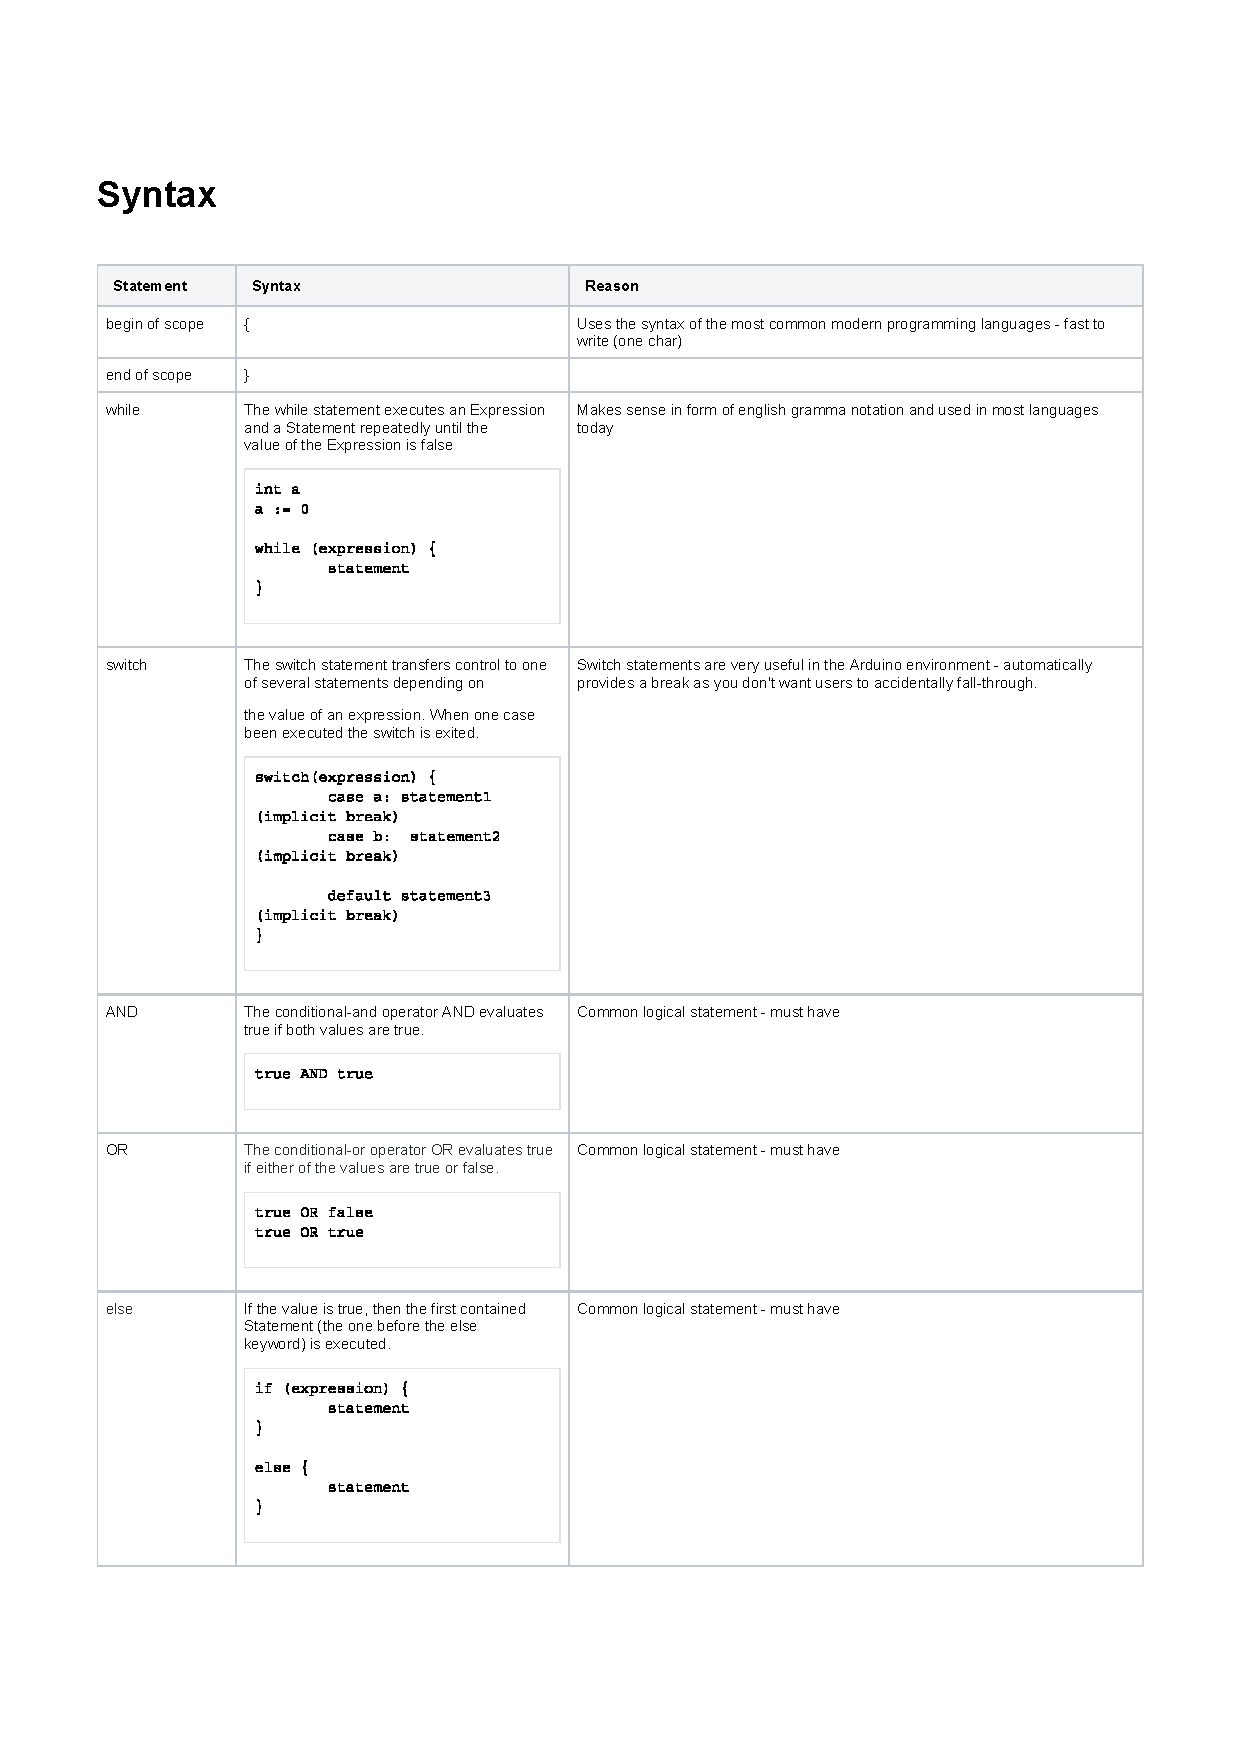
\includepdf[scale=1.0, pagecommand={}]{sections/analysis/pdf/Syntax1.pdf}
 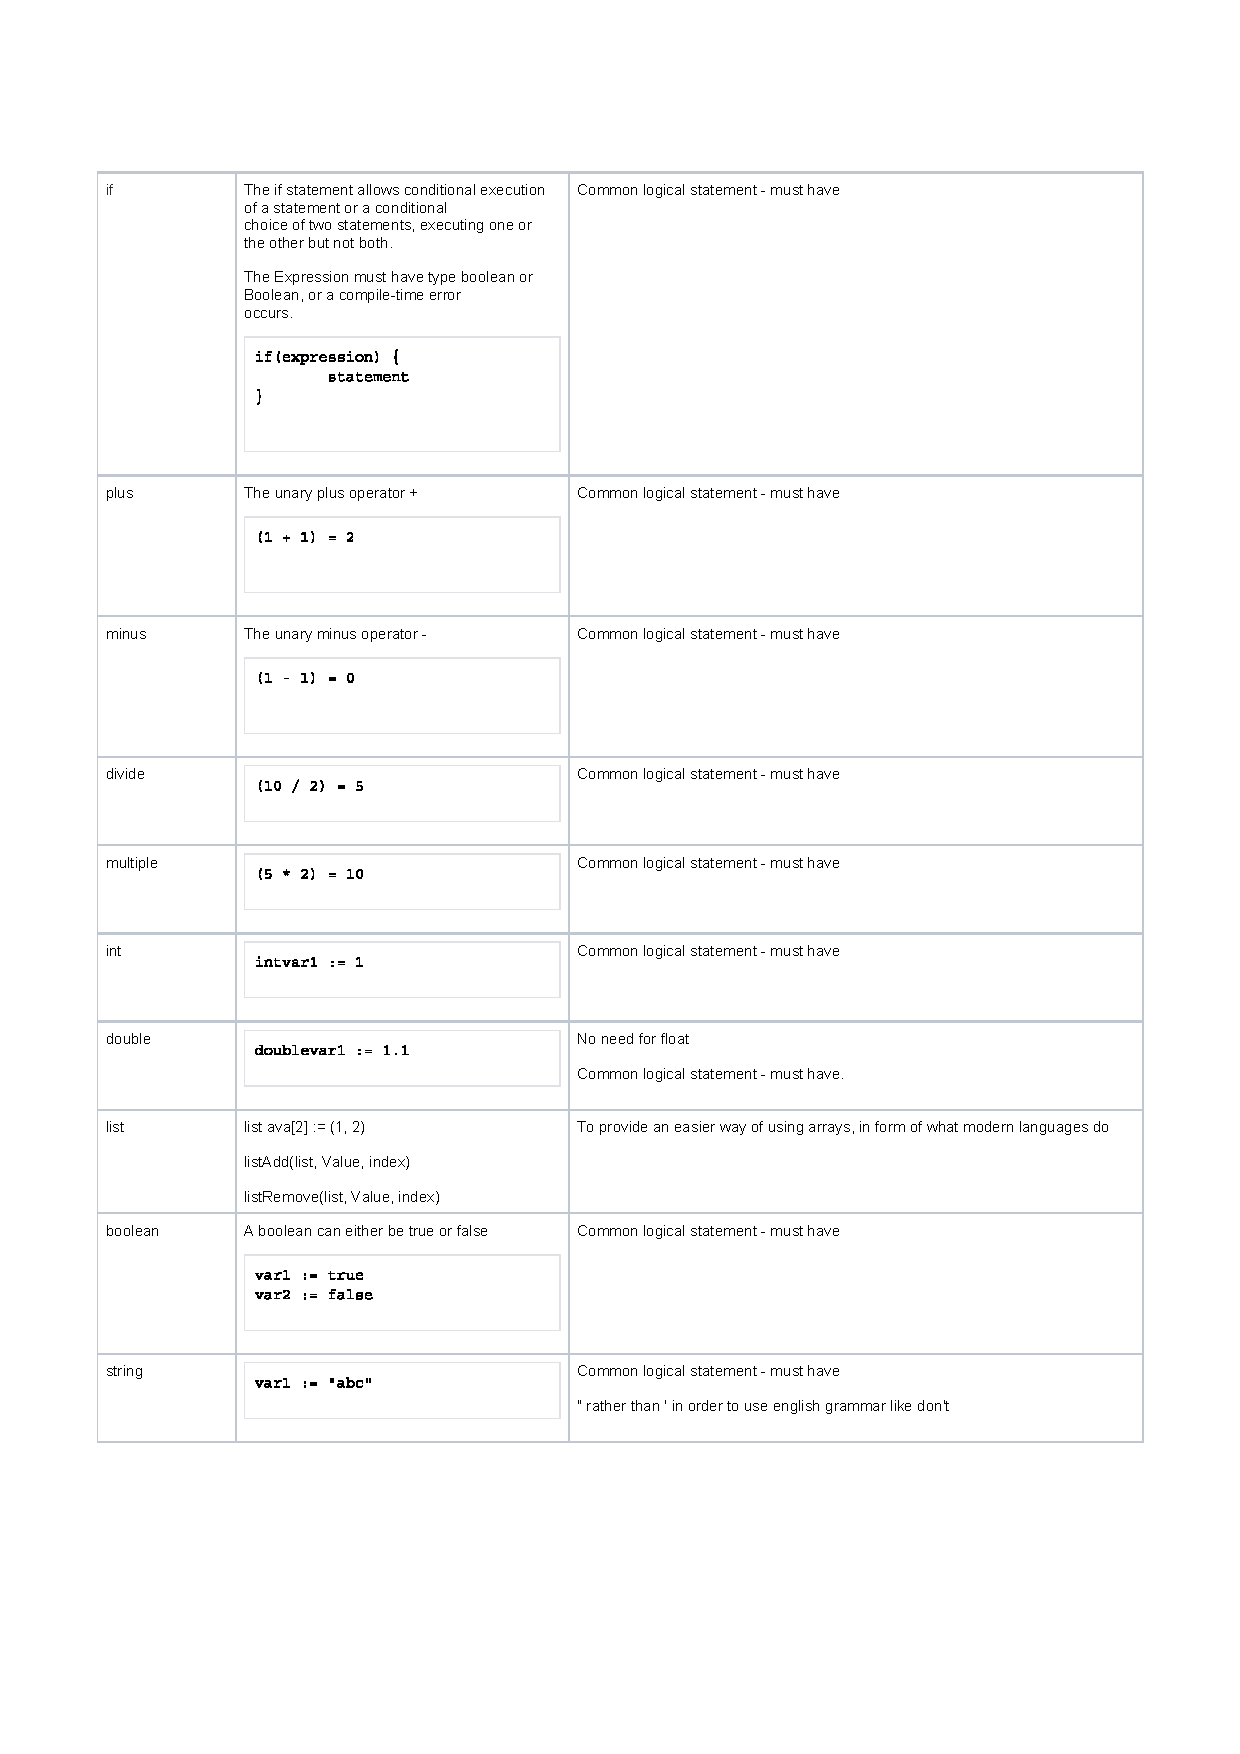
\includepdf[scale=1.0, pagecommand={}]{sections/analysis/pdf/Syntax2.pdf}  
 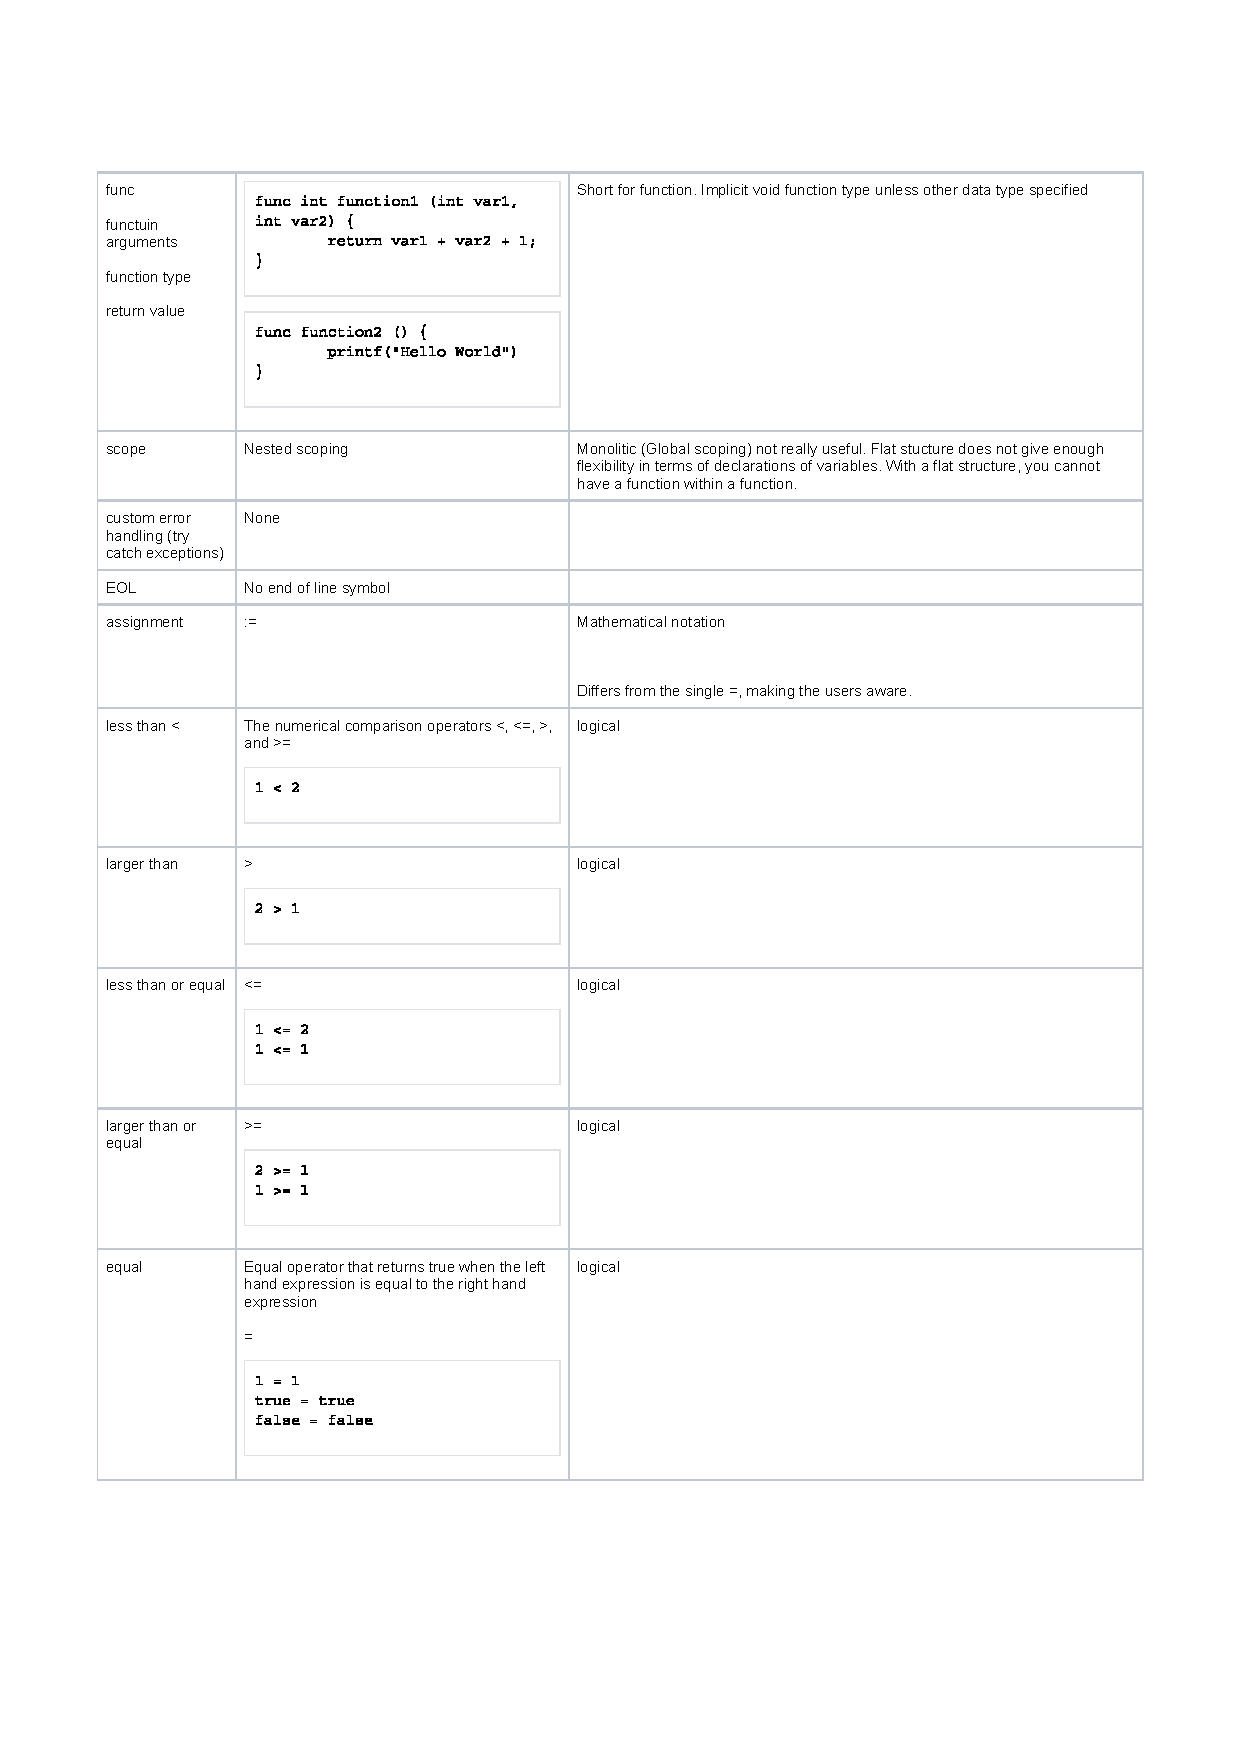
\includepdf[scale=1.0, pagecommand={}]{sections/analysis/pdf/Syntax3.pdf}  
 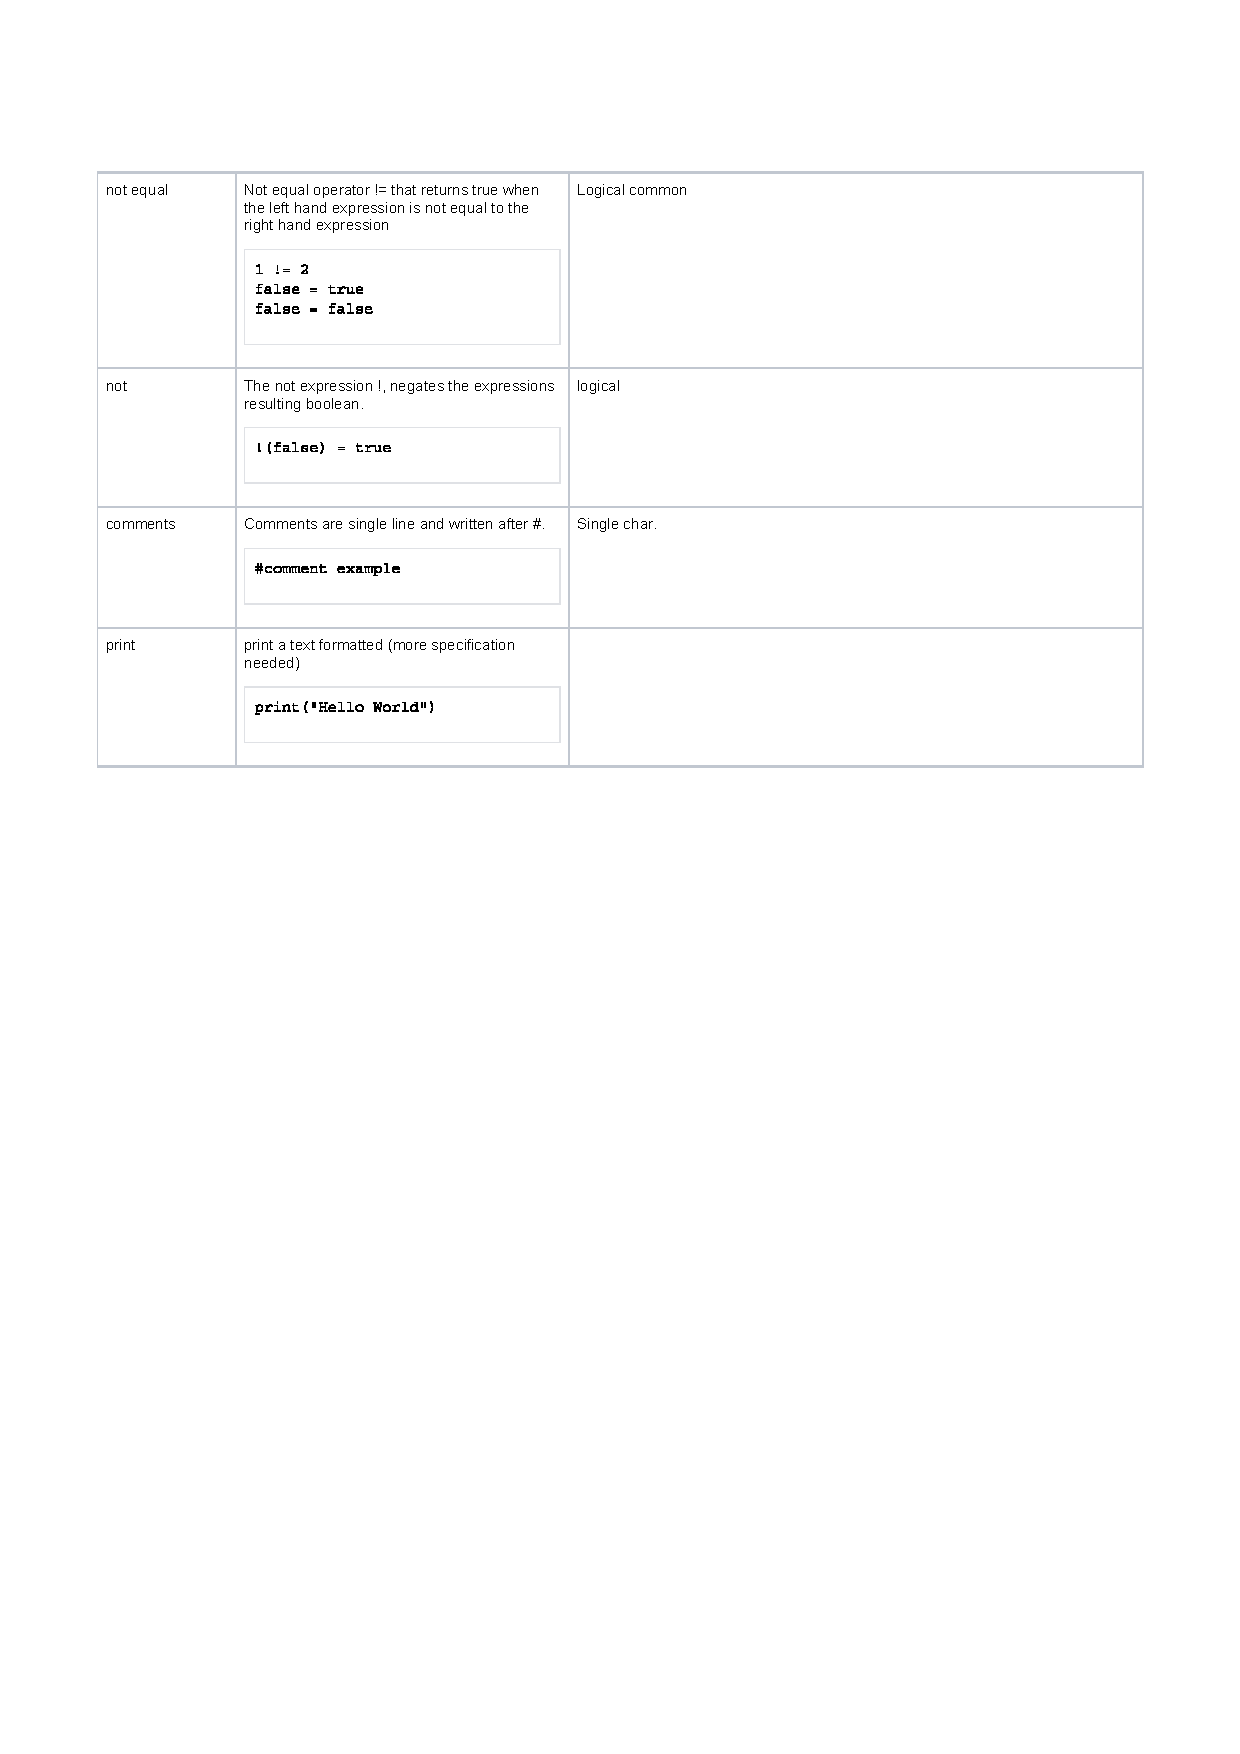
\includepdf[scale=1.0, pagecommand={}]{sections/analysis/pdf/Syntax4.pdf}  

 
 %\\\\
In Java and C for whenever a block of code was finished it would have a ; operator at the end of the line, but in the project's language there would be no ; at the end of the line because if one is not aware of what he is writing, he would easily forget to set the ; at the end of the line. That is why the language will not include ;. \\
 \\
All the conditional operators have been spelled with capital letters. The reason for this is. so the conditional operators can be distinguished from the conditions and variables. \\
 \\
The next part are the beginning and end of the scope, which will keep it's {} at the beginning and the end of the scope just like C.  \\
 \\
The if and else conditions will stay the same as they are in both C and Java because it is not complicated. \\
 \\
All mathematics operations will be the same as they are, to ensure no confusions can be made when using those operators. \\
 \\
When a variable needs to get its value the assignment := will be used to showcase the variable's value. The numerical comparison operators will use something similar with the  larger/less or equal operation, which looks like this >= or <=. The larger or less will always be on the left side to ensure no confusion for the user, when using them. It is also to make the assignment to be more mathematical and it is the same as the one pascal uses.  \\
 \\
The not expression !, will stay the same as it is, just like Java and C. \\
 \\
To comment in the language the user must write after a \# to make comment. The \# will only make a comment for a single line so if the user wanted to write a comment that is two lines long the user must do it like this.
\#Hello
\#world \\
 \\
To print a string or something else one must use the print function, which is just like C.\\
 \\
The while and switch statement, follows the same principles as the C programming language, since they are used the same way in the Arduino enviroment.\\
 \\
Compared to the Common logical statement, the boolean statements will be in small letters to differentiate them from the other logical statements, this means to use the boolean statements, one must write true or false instead of TRUE or FALSE.\\
 \\
 Int and doubles will be used in the programming language, while not using something like float, because it would not be needed in the programming language environment, which is home automation
 
  This section will go through the decision on how the programming language was designed.
 \\
 The design phases are the following: making the new programming language uphold the criteria for designing a programming language for readability, writeability and reliability, 
 